\documentclass[../main.tex]{subfiles}

\makeatletter
\@ifundefined{fromRoot}{%
  \newcommand{\fromRoot}[1]{../#1}
  
 % \usepackage{xr}
  % \externaldocument{../main}
}{}

\def\input@path{{\subfix{../}}}
%or: \def\input@path{{/path/to/folder/}{/path/to/other/folder/}}
\makeatother

\graphicspath{
  {\subfix{../}}
  {\subfix{./figures}}
  {\subfix{../figures}}
  {\subfix{./figures/logos-thesis/}}
  {\subfix{../figures/logos-thesis/}}
  {\subfix{./figures/rtexps-pics/}}
  {\subfix{../figures/rtexps-pics/}}
}

\hypersetup{
    pdfauthor   = {Camille MONIÈRE},
    pdftitle    = {Th\`{e}se (Présentation: Back-Ups)},
    pdfsubject  = {Th\`{e}se (Présentation: Back-Ups)},
%    pdfkeywords = {mots-cl\'{e}s},
}

\begin{document}

\section*{Back-Ups}

\subsection*{\acrfull{lpwan}}

\begin{frame}{\acrshortpl{lpwan}}
  \begin{columns}
    \begin{column}{.5\linewidth}
      \includegraphics[width=\linewidth, height=.65\textheight, keepaspectratio=true]{figures/tikzpicture/topo-network.pdf}
      \captionof{figure}{Topologie possible d'un \acrshort{lpwan}.}
    \end{column}
    \begin{column}{.5\linewidth}
      Composition du réseau :

      \begin{ctrlitemize}{2pt}
        \item [\textcolor{RoyalBlue3}{$\bullet$}] \textcolor{RoyalBlue3}{Nœud-capteurs   }
        --- bon-marchés, fonctionnant sur batterie, déployables massivement.
        \item [\textcolor{Chartreuse3}{$\blacklozenge$}] \textcolor{Chartreuse3}{Relais  }
        --- plus cher que les nœud-capteurs, mais plus performants.
        \item [\textcolor{Gold3}{$\blacksquare$}] \textcolor{Gold3}{Stations de base     }
        --- couteuses et très performantes, mais en nombre réduit.
      \end{ctrlitemize}
    \end{column}
  \end{columns}
\end{frame}


\subsection{Émission : fonctionnellement simple}

\begin{frame}{\subsecname}
  \begin{columns}
    \begin{column}{.35\linewidth}
      \begin{overlayarea}{\linewidth}{.5\textheight}
        \centering
        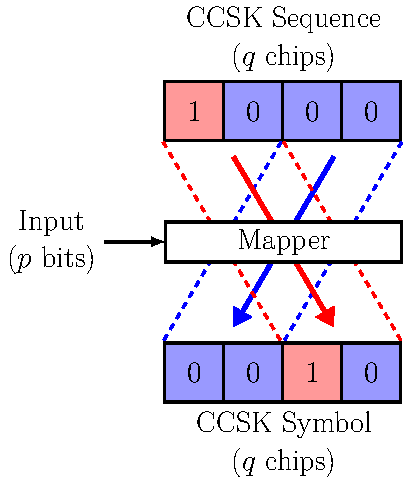
\includegraphics[width=\linewidth, height=.5\textheight, keepaspectratio = true]{figures/tikzpicture/ccsk_simd_stdl.pdf}
        \captionof{figure}{Modulation CCSK, en image.}
      \end{overlayarea}
    \end{column}
    \begin{column}{.35\linewidth}
      \begin{overlayarea}{\linewidth}{.5\textheight}
        \centering
        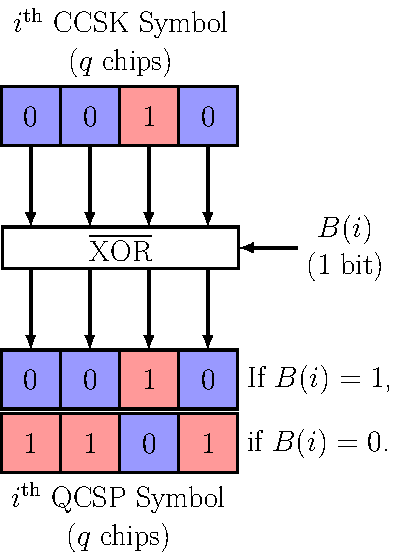
\includegraphics[width=\linewidth, height=.55\textheight, keepaspectratio = true]{figures/tikzpicture/ovmod_simd_stdl.pdf}
        \captionof{figure}{Surmodulation, en image.}
      \end{overlayarea}
    \end{column}
  \end{columns}

  \vspace{4 em}

  \begin{center}
    Le NB-LDPC et le filtre sont des fonctions très étudiées dans la littérature.
  \end{center}
\end{frame}


\subsection*{Étude de la norme}
\begin{frame}{\subsecname}
  \begin{columns}
    \begin{column}{.9 \linewidth}
      \centering
      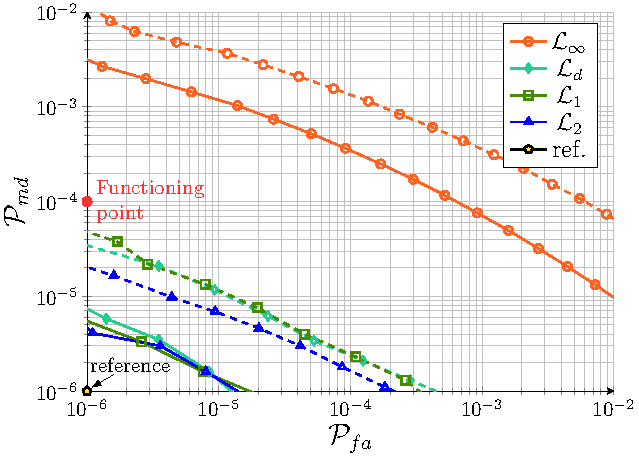
\includegraphics[height = .8\textheight]{pgfplots/roc_curves_norms_stdl.pdf}
    \end{column}
  \end{columns}
\end{frame}

\subsection*{Variation de corrélations : Complexité}

\begin{frame}
  \frametitle{\subsecname}

  \scriptsize \centering
  \captionof{table}{Complexité calculatoire pour $\textcolor{red}{\mpd}$ corrélations des méthodes FFT et TS avec $\textcolor{blue}{p_\omega = 1}$ .}
  % \begin{noindent}
  \begin{tabular}{@{}r r @{\phantom{XX}} r @{\phantom{XX}} r @{\phantom{XX}} r@{}}
\toprule
\ra{1.4}        & $\bm{\textcolor{red}{\mpd}}$
        & \textbf{Add}
        & \textbf{Multiply}
        & \textbf{Memory}                              \\
\midrule
\textbf{\fft{}} & $\llbracket 1, \; q - 1 \rrbracket$ 
        & $2 \textcolor{red}{\mpd} q \log_2(q)$
        & $\textcolor{red}{\mpd} q(\log_2(q) + 2)$
        & $(\frac{\textcolor{red}{\mpd} - 1}{\textcolor{red}{\mpd}} + \textcolor{red}{\mpd})q$ \\
              & $q$                                 
        & $2 q^2 \log_2(q)$
        & $q^2(\log_2(q) + 2)$
        & $q^2 + q + 1$                                 \\
                      \cmidrule{2-5}
\textbf{\ts{}}  & $q$
                & $q^2 + q$
                & $q^2$
                & $2q$                                   \\
\bottomrule
  \end{tabular}
  % \end{noindent}
  \ra{1}

\end{frame}

\subsection*{Parallélisme}
\begin{frame}[fragile]{SPMD : Exemple --- Somme de $10^9$ valeurs en C}
  \begin{columns}
    \begin{column}{.33\linewidth}
      \begin{overlayarea}{\linewidth}{.87\textheight}
        \centering
        \textbf{Séquentielle en C}\\\textit{\phantom{OpenMP}} \vspace{.00\textheight}

        \begin{lstlisting}[style=cstyle,basicstyle=\tiny]
  int64_t sum = 0;
  for (int i = 0; i < (int) 1e9; i++) {
    sum += i;
  }\end{lstlisting}
      \end{overlayarea}
    \end{column}
    \begin{column}{.33\linewidth}
      \begin{overlayarea}{\linewidth}{.87\textheight}
        \centering
        \textbf{Parallèle en C}\\\textit{\phantom{p}à la main\phantom{O}} \vspace{.00\textheight}

        \begin{lstlisting}[style=cstyle,basicstyle=\tiny]
  struct ptarg {int64_t sum, int begin};
  int max = ((int) 1e9) / 4;
  
  void * func(void * in){
    struct ptarg * arg = in; 
    for (int i = arg->begin; i < max; i++) {
      arg->sum += i;
    }
  }
  
  struct ptarg args[4];
  pthread_t    ths[4];
  
  for (int i = 0; i < 4; i++) {
    args[i] = {0, i};
    pthread_create(
      ths + i, NULL, func, args + i
    );
  }
  
  int64_t sum = 0;
  for (int i = 0; i < 4; i++) {
    pthread_join(ths + i);
    sum += args[i].sum;
  }\end{lstlisting}
      \end{overlayarea}
    \end{column}
    \begin{column}{.33\linewidth}
      \begin{overlayarea}{\linewidth}{.87\textheight}
        \centering
        \textbf{Parallèle en C}\\\textit{OpenMP} \vspace{.00\textheight}

        \begin{lstlisting}[style=cstyle,basicstyle=\tiny]
  int64_t sum = 0;
  #pragma omp parallel for reduction(+:sum)
  for (int i = 0; i < (int) 1e9; i++) {
    sum += i;
  }\end{lstlisting}
      \end{overlayarea}
    \end{column}
  \end{columns}
\end{frame}

\subsection*{Perspectives}
\begin{frame}{\subsecname{} II}
  \begin{columns}
    \begin{column}{.9 \linewidth}
      \centering
      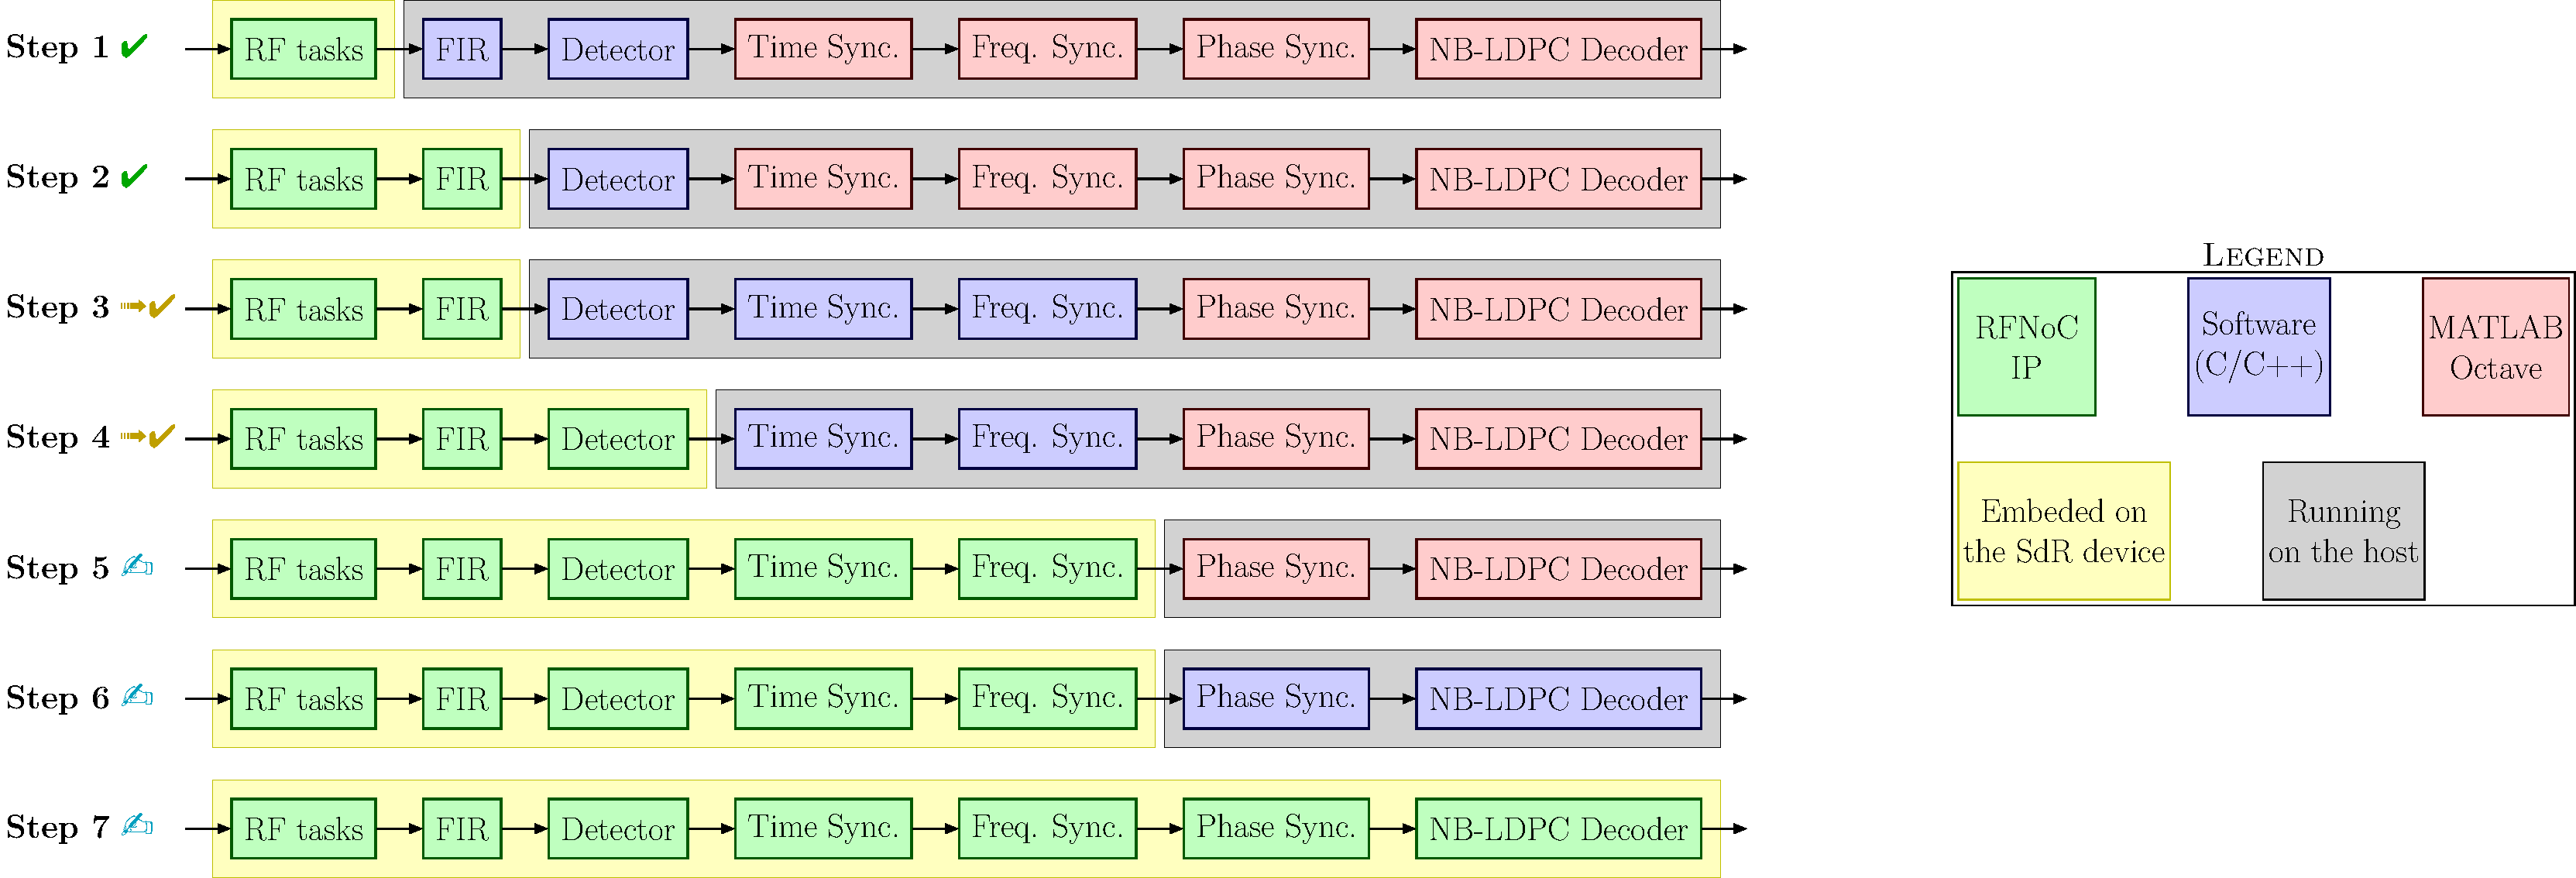
\includegraphics[width = \linewidth]{tikzpicture/implementation_tasks_stdl.pdf}
      \captionof{figure}{Plan prévisionnel de développement pour un récepteur QCSP tout-en-un embarqué.}
    \end{column}
  \end{columns}
\end{frame}

\end{document}
